\documentclass[11pt]{beamer}
\usetheme{default}

\usepackage[utf8]{inputenc}
\usepackage[T1]{fontenc}
\usepackage{amsmath}
\usepackage{amsfonts}
\usepackage{amssymb}
\usepackage{graphicx}
\usepackage{tikz}
\usepackage{filecontents}
\usepackage{pgfplots}

\author{Marek Kidoň}
\title{Evolutionary design of domain specific non-cryptographic hash functions}

\subtitle{}

\logo{}

\institute{Brno University of Technology}

\date{\today}

\subject{}

\setbeamercovered{transparent}

\setbeamertemplate{navigation symbols}{}

\setbeamerfont{page number in head/foot}{size=\large}
\setbeamertemplate{footline}[frame number]

\begin{document}
	\begin{frame}[plain]
		\titlepage
		 \addtocounter{framenumber}{-1}
	\end{frame}
	\begin{frame}
		\frametitle{Hash function [1/2]}
		\begin{block}{Introduction} 
		\begin{itemize}[<+->]
			\item Function of form $f_{hash} : U \to S$ for virtually any  key universe $U$ and $S = \{ 0,1,2 \ldots n \}$.
			\item $|U| \gg |S|$.
			\item Collision: $f_{hash}(k_1) = f_{hash}(k_2)$ pro $k_1, k_2 \in U, k_1 \neq k_2$.
			\item One of the most important applications are hash tables and cryptography.
			\item State of the art implementations: \textit{lookup3}, \textit{Murmurhash3}, \textit{CityHash}, \textit{FarmHash}
		\end{itemize}
		\end{block}
	\end{frame}
	
	\begin{frame}
		\frametitle{Hash function [2/2]}
		\begin{block}{Idea} 
			\begin{itemize}[<+->]
				\item Domain specific vs. generic hash functions. \\
				\item Idea : ``Tailor suiting'' hash function to a specific domain leads to a better performance in terms of
					\textit{collision resistance}. 
			\end{itemize}
		\end{block}
		\begin{figure}
		\centering
		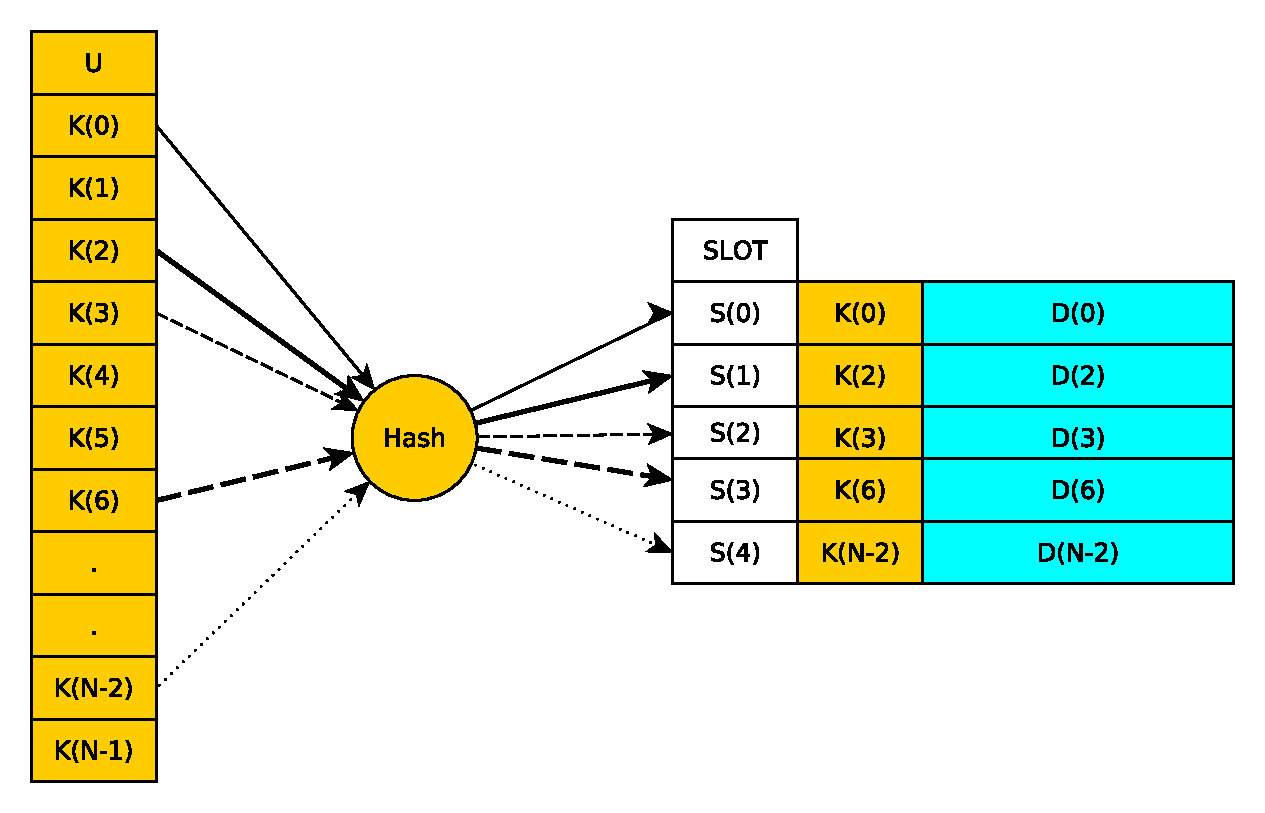
\includegraphics[height=5cm]{fig/hash_table_example}
		\caption{Hash table example}
		\end{figure}
	\end{frame}
	
	\begin{frame}
		\frametitle{Evolution Design}
		\begin{block}{An unconventional approach}
			\begin{itemize}[<+->]
				\item Vast variety of problems can be view as state space search problem.
				\item Inspired by the process of species reproduction.
				\item It is typically implemented as an iterative algorithm (evolutionary algorithm).
			\end{itemize}
		\end{block}
		\begin{block}{Evolution algorithm}
			\begin{itemize}[<+->]
				\item Uses a \textit{population} to represent a set of feasible solutions called \textit{individual}.
				\item New generation is bred by selecting \textit{fit} individuals using a \textit{fitness function} 
					and applying \textit{genetic operators}.
			\end{itemize}  
		\end{block}
	\end{frame}
	
	\begin{frame}
		\frametitle{Problem specification}
		\begin{itemize}[<+->]
				\item The target domain are \textit{Internet Protocol} (IP) version 4 addresses.
				\item Four different IP datasets are specified.
				\item Evolutionary design a hash function for each subset such that it outperforms
					human-created solutions.
		\end{itemize}
	\end{frame}
	\begin{frame}{Solution design}
		\begin{columns}[T]
			\begin{column}{7cm}
			\begin{itemize} [<+->]
				\item \textit{Genetic programming} (GP) evolutionary algorithm
				\item Individuals are represented as \textit{abstract syntax trees}.
				\item Nodes are commonly used hashing operators such as the multiplication ($*$), addtition ($+$) or rotation ($\lll$).
				\item Leafs are IP address octets ($o_0, o_1, o_2, o_3$) and randomly selected prime numbers ($\Re$).
				\item Fitness function measures how many collision free addresses individual hashes. Bigger number means better individual.
			\end{itemize}
			\end{column}
			\begin{column}{5cm}
				\begin{figure}
					\centering
					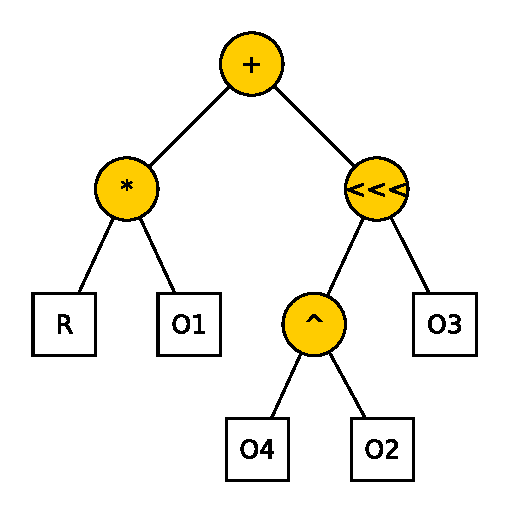
\includegraphics[height=5cm]{fig/ast_example}
					\caption{GP individual example}
				\end{figure}
			\end{column}
		\end{columns}
	\end{frame}
	\begin{frame}{Results}
		
	\begin{figure}[!ht]
		\centering
		\begin{tikzpicture}
		\begin{axis}[ %
		, name=plot1
		, height=6.4cm
		, width=10cm
		, grid=major
		, xlabel=Generation
		, ymin=5180
		, ymax=5320
		, ylabel=Successfully hashed
		, legend style=
		{ at={(1.0, 0.3)}
			, anchor=east
		}
		]
		\addplot[color=black, dashdotted, thick, mark=none] table {graph/ElitistRandomRun.dat};
		\addlegendentry{Elitist Random Search}
		
		\addplot[color=blue, dotted, very thick, mark=none] table {graph/RandomRun.dat};
		\addlegendentry{Random Search}
		
		\addplot[color=green, solid, thick, mark=none] coordinates {(0,5190) (194, 5190)};
		\addlegendentry{MurmurHash3}
		
		\addplot[color=red, mark=none, dashed, thick] table {graph/IPHashMedian.dat}; 
		\addlegendentry{Proposed IPHash}
		\end{axis}
	\end{tikzpicture}
	\end{figure}
	
	\begin{multline}
	f_{o_0, o_1, o_2, o_3} = (((\Re \wedge (o_1 \wedge o_3)) + (o_2 * \Re)) + \\
	((\Re \ggg o_1) \ggg (((o_1 * o_0) \ggg o_1) * (\Re \ggg o_1))))
	\label{eq:hash}
	\end{multline}
	\end{frame}
	\begin{frame}{Conclusion}
		We found hash functions such that they outperform human created ones considering the given dataset.
		\begin{block}{There is always a room for an improvement}
			\begin{itemize}
				\item No collision resolution mechanism was used\ldots
				\item No hash function construction scheme was incorporated in the design.
			\end{itemize}
		\end{block}		
	\end{frame}
	\begin{frame}{References}
		Luk\'{a}\v{s} Sekanina. \textit{Evolu\v{c}n\'{i} hardware}. Academia, 2009. \\~\\
		
		Mustafa Safdari. Evolving universal hash functions using genetic algorithms.
		In \textit{Proceedings of the 11th Genetic and Evolutionary Computation Conference}, page 2729–2732, New York, 2009. \\~\\
		
		C\'{e}sar Est\'{e}banez, Yugo Saez, Gustavo Recio and Pedro Isasi. Automatic design of non-cryptographic hash functions using 
		genetic programming. \textit{Computational Intelligence}. 30(4):798-831, 2014. \\~\\
		
		Roland Dobai and Jan Ko\v{r}enek. Evolution of non-cryptographic hash function pairs for fpga-based network applications. In 
		\textit{2015 IEEE Symposium Series on Computational Intelligence}, pages 1214-1219. Institute of Electrical and Electronis Engineers, 2015.
	\end{frame}		
\end{document}